% Source: tex/chapters/ch06/05_ソフトウェアエンジニアリング運用計画.tex
\paragraph{運用計画}

運用計画は、プロジェクト要求、開発者や保守担当者のニーズを、運用サービスへ翻訳する活動である。開発は数か月から数年で終わることが多いが、運用は何年も続く。そのため、資源見積もり、人員計画、教育、予算、容量、支援体制を早くから考えることが重要である。

新しいソフトウェアを開発すると決めた時点で、運用と保守の要求を考慮すべきである。概念文書、運用保守計画、運用構想（Concept of Operations, CONOPS）を作り、利用者が変更要求や問題報告をどのように出すか、誰が受け付けるか、どのように優先順位を付けるか、どのようにリリースへ反映するかを明らかにする。

\par\smallskip\noindent\refstepcounter{table}\label{tab:ch06-04}\textbf{表 \thetable: 第06章 ソフトウェアエンジニアリング運用 表04}\par\smallskip
\begin{longtable}{L{45mm}L{105mm}}
\toprule
運用計画で扱う項目 & 説明 \\
\midrule
役割と責任 & 新しいサービスまたは変更されたサービスを、誰が実装、運用、保守するかを決める。 \\
顧客と供給者の活動 & 顧客側と供給者側が行う作業、契約、合意を明確にする。 \\
要員と教育 & 必要な人員、技能、訓練、技術支援を計画する。 \\
プロセスとツール & 使う手順、測定、方法、ツールを定義する。 \\
容量と財務 & 将来の利用量、予算、時程、費用を見積もる。 \\
サービス受け入れ基準 & 運用開始できると判断する条件を決める。 \\
期待成果 & 運用した結果として何を測定し、どの水準を満たすかを数値で表す。 \\
\bottomrule
\end{longtable}

個々の問題報告や変更要求のレベルでは、対象となるリリース日、次版の内容、潜在的な衝突、リスク、ロールバック計画、データ移行計画、関係者への通知を扱う。

\begin{figure}[htbp]
\centering
\IfFileExists{assets/generated_figures/ch06/fig-ch06-03.png}{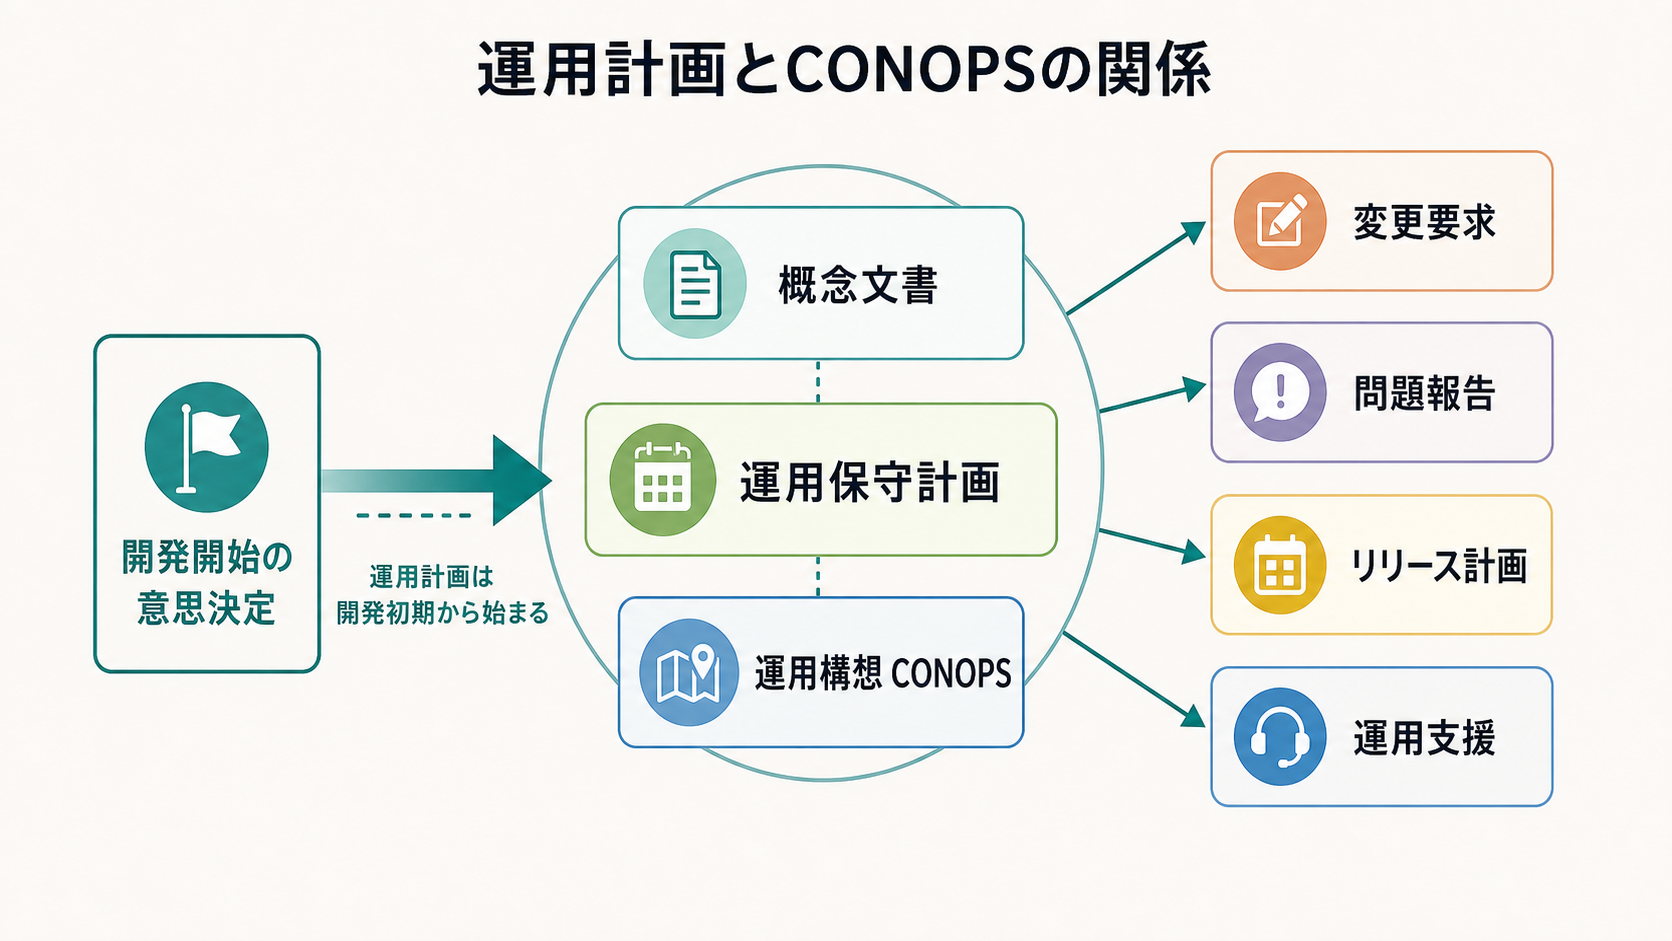
\includegraphics[width=0.96\linewidth]{assets/generated_figures/ch06/fig-ch06-03.png}}{\fbox{\parbox[c][48mm][c]{0.9\linewidth}{\centering 画像生成待ち\\運用計画とCONOPSの関係}}}
\caption{運用計画とCONOPSの関係}
\label{fig:ch06-03}
\end{figure}
